% A block of five consecutive integers and the coprime pairs inside it.
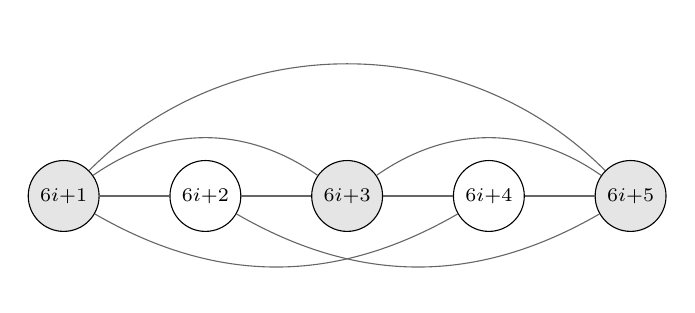
\begin{tikzpicture}[
  od/.style={circle, draw=black, fill=black!10, minimum size=9mm, font=\scriptsize, inner sep=0pt},
  ev/.style={circle, draw=black, fill=white, minimum size=9mm, font=\scriptsize, inner sep=0pt},
  e/.style={black!60}]
\node[od] (a) at (0,0) {$6i{+}1$};
\node[ev] (b) at (1.8,0) {$6i{+}2$};
\node[od] (c) at (3.6,0) {$6i{+}3$};
\node[ev] (d) at (5.4,0) {$6i{+}4$};
\node[od] (f) at (7.2,0) {$6i{+}5$};
\draw[e] (a) to[bend left=35] (c);
\draw[e] (c) to[bend left=35] (f);
\draw[e] (a) to[bend left=45] (f);
\draw[e] (a) -- (b);
\draw[e] (b) -- (c);
\draw[e] (c) -- (d);
\draw[e] (d) -- (f);
\draw[e] (a) to[bend right=30] (d);
\draw[e] (b) to[bend right=30] (f);
\end{tikzpicture}
